% Final report, ECE 425-525 course project P04. Same look as the proposal
% (Agentic_AI_VLSI_Proposal.tex). Compiles with pdflatex (Overleaf's default).
%
%   python docs/final-report/generate.py     # tables, chart data and numbers from runs/bench/
%   cd docs/final-report && latexmk -pdf report.tex
%
% Numbers in the text come from \fact{key} (generated/facts.tex), never typed by hand;
% a mistyped key prints in red. Blue boxes are the parts still to be written.

\documentclass[11pt,a4paper]{article}

% --- Preamble from the proposal ---
\usepackage[a4paper,top=2.5cm,bottom=2.5cm,left=2cm,right=2cm]{geometry}
\usepackage[T1]{fontenc}
\usepackage[utf8]{inputenc}
\usepackage[english]{babel}
\usepackage{helvet}
\renewcommand{\familydefault}{\sfdefault}
\usepackage{enumitem}
\usepackage{amssymb}
\usepackage{xcolor}
\usepackage{colortbl}
\usepackage{parskip}
\usepackage{titlesec}
\usepackage{needspace}
\usepackage{tabularx}
\usepackage{tikz}
\usetikzlibrary{arrows.meta,positioning,calc}
\usepackage{hyperref}

% --- Added for the report ---
\usepackage{booktabs}
\usepackage{makecell}
\usepackage{caption}
\usepackage{float}
\usepackage{fvextra}  % fancyvrb plus line wrapping, for the prompts in the appendix
\usepackage{pgfplots}
\pgfplotsset{compat=1.18, /pgf/number format/assume math mode=true}  % numbers in the text font, not serif math

\definecolor{boxfill}{RGB}{238,243,248}
\definecolor{arrowcolor}{RGB}{70,100,140}
\definecolor{primary}{RGB}{30,64,120}
\definecolor{secondary}{RGB}{70,90,120}
\definecolor{accent}{RGB}{245,247,250}
\definecolor{border}{RGB}{200,210,225}
\definecolor{good}{RGB}{30,120,60}
\definecolor{bad}{RGB}{170,40,40}
\definecolor{todo}{RGB}{40,90,170}

\titleformat{\section}{\Large\bfseries\color{primary}}{\thesection.}{0.5em}{}[\titlerule]
\titleformat{\subsection}{\large\bfseries\color{secondary}}{\thesubsection}{0.5em}{}
\titlespacing*{\section}{0pt}{14pt}{7pt}
\setlength{\parskip}{5pt}
\setlength{\emergencystretch}{2em}
\setlist[itemize]{leftmargin=1.4em,itemsep=3pt,topsep=3pt}
\captionsetup{font=small,labelfont={bf,color=primary}}

\hypersetup{colorlinks=true, linkcolor=primary, urlcolor=primary, citecolor=primary,
  pdftitle={VLSI Design Agent: Final Report}, pdfauthor={Course Project Team P04}}

% The proposal's framed answer box.
\newcommand{\answerbox}[1]{%
  \par\smallskip\begingroup\setlength{\fboxsep}{6pt}%
  \noindent\fcolorbox{border}{accent}{\parbox{\dimexpr\linewidth-2\fboxsep-2\fboxrule\relax}{\small\raggedright #1}}%
  \par\endgroup\smallskip}

% Numbers from the runs; an unknown key shows up in red.
% Generated by generate.py from runs/bench/. Use \fact{key} in report.tex.
\makeatletter
\expandafter\def\csname fact@both-default-final\endcsname{48/50}
\expandafter\def\csname fact@both-default-oneshot\endcsname{46/50}
\expandafter\def\csname fact@both-final-range\endcsname{45--48/50}
\expandafter\def\csname fact@both-sfone-final\endcsname{45/50}
\expandafter\def\csname fact@both-sfone-oneshot\endcsname{43/50}
\expandafter\def\csname fact@both-sftwo-final\endcsname{46/50}
\expandafter\def\csname fact@both-sftwo-oneshot\endcsname{43/50}
\expandafter\def\csname fact@both-tbtiming-final\endcsname{47/50}
\expandafter\def\csname fact@both-tbtiming-oneshot\endcsname{48/50}
\expandafter\def\csname fact@broken\endcsname{4}
\expandafter\def\csname fact@budget\endcsname{50,000}
\expandafter\def\csname fact@circuits\endcsname{10}
\expandafter\def\csname fact@dev-default-broken\endcsname{0}
\expandafter\def\csname fact@dev-default-final\endcsname{24/25}
\expandafter\def\csname fact@dev-default-fixed\endcsname{0}
\expandafter\def\csname fact@dev-default-oneshot\endcsname{24/25}
\expandafter\def\csname fact@dev-default-rejected\endcsname{51\%}
\expandafter\def\csname fact@dev-default-tokens\endcsname{7,296}
\expandafter\def\csname fact@dev-rejected-range\endcsname{21--51\%}
\expandafter\def\csname fact@dev-sfone-broken\endcsname{0}
\expandafter\def\csname fact@dev-sfone-final\endcsname{24/25}
\expandafter\def\csname fact@dev-sfone-fixed\endcsname{1}
\expandafter\def\csname fact@dev-sfone-oneshot\endcsname{23/25}
\expandafter\def\csname fact@dev-sfone-rejected\endcsname{21\%}
\expandafter\def\csname fact@dev-sfone-tokens\endcsname{5,985}
\expandafter\def\csname fact@dev-sftwo-broken\endcsname{2}
\expandafter\def\csname fact@dev-sftwo-final\endcsname{23/25}
\expandafter\def\csname fact@dev-sftwo-fixed\endcsname{2}
\expandafter\def\csname fact@dev-sftwo-oneshot\endcsname{23/25}
\expandafter\def\csname fact@dev-sftwo-rejected\endcsname{32\%}
\expandafter\def\csname fact@dev-sftwo-tokens\endcsname{6,744}
\expandafter\def\csname fact@dev-tbtiming-broken\endcsname{1}
\expandafter\def\csname fact@dev-tbtiming-final\endcsname{22/25}
\expandafter\def\csname fact@dev-tbtiming-fixed\endcsname{0}
\expandafter\def\csname fact@dev-tbtiming-oneshot\endcsname{23/25}
\expandafter\def\csname fact@dev-tbtiming-rejected\endcsname{36\%}
\expandafter\def\csname fact@dev-tbtiming-tokens\endcsname{5,906}
\expandafter\def\csname fact@fixed\endcsname{10}
\expandafter\def\csname fact@fixtures\endcsname{58}
\expandafter\def\csname fact@fixtures-correct\endcsname{20}
\expandafter\def\csname fact@heldout-default-broken\endcsname{0}
\expandafter\def\csname fact@heldout-default-final\endcsname{24/25}
\expandafter\def\csname fact@heldout-default-fixed\endcsname{2}
\expandafter\def\csname fact@heldout-default-oneshot\endcsname{22/25}
\expandafter\def\csname fact@heldout-default-rejected\endcsname{81\%}
\expandafter\def\csname fact@heldout-default-tokens\endcsname{10,501}
\expandafter\def\csname fact@heldout-rejected-range\endcsname{54--81\%}
\expandafter\def\csname fact@heldout-sfone-broken\endcsname{1}
\expandafter\def\csname fact@heldout-sfone-final\endcsname{21/25}
\expandafter\def\csname fact@heldout-sfone-fixed\endcsname{2}
\expandafter\def\csname fact@heldout-sfone-oneshot\endcsname{20/25}
\expandafter\def\csname fact@heldout-sfone-rejected\endcsname{65\%}
\expandafter\def\csname fact@heldout-sfone-tokens\endcsname{12,526}
\expandafter\def\csname fact@heldout-sftwo-broken\endcsname{0}
\expandafter\def\csname fact@heldout-sftwo-final\endcsname{23/25}
\expandafter\def\csname fact@heldout-sftwo-fixed\endcsname{3}
\expandafter\def\csname fact@heldout-sftwo-oneshot\endcsname{20/25}
\expandafter\def\csname fact@heldout-sftwo-rejected\endcsname{59\%}
\expandafter\def\csname fact@heldout-sftwo-tokens\endcsname{12,817}
\expandafter\def\csname fact@heldout-tbtiming-broken\endcsname{0}
\expandafter\def\csname fact@heldout-tbtiming-final\endcsname{25/25}
\expandafter\def\csname fact@heldout-tbtiming-fixed\endcsname{0}
\expandafter\def\csname fact@heldout-tbtiming-oneshot\endcsname{25/25}
\expandafter\def\csname fact@heldout-tbtiming-rejected\endcsname{54\%}
\expandafter\def\csname fact@heldout-tbtiming-tokens\endcsname{6,780}
\expandafter\def\csname fact@max-attempts\endcsname{3}
\expandafter\def\csname fact@model\endcsname{gemma4:26b}
\expandafter\def\csname fact@runs\endcsname{200}
\expandafter\def\csname fact@seeds\endcsname{1--5}
\expandafter\def\csname fact@temperature\endcsname{0.2}
\makeatother

\newcommand{\fact}[1]{\ifcsname fact@#1\endcsname\csname fact@#1\endcsname\else\textcolor{red}{\textbf{[#1?]}}\fi}
\newcommand{\up}[1]{\textcolor{good}{#1}}
\newcommand{\down}[1]{\textcolor{bad}{#1}}

% Still to write: remove each box once its section is done.
\newcommand{\todo}[1]{%
  \par\smallskip\begingroup\setlength{\fboxsep}{5pt}%
  \noindent\fcolorbox{todo}{todo!6}{\parbox{\dimexpr\linewidth-2\fboxsep-2\fboxrule\relax}{\small
    \textbf{\textcolor{todo}{To write:}} #1}}%
  \par\endgroup\smallskip}
% A screenshot to take from the dashboard.
\newcommand{\shot}[2]{%
  \begin{figure}[H]\centering
    \fcolorbox{border}{accent}{\parbox[c][4.2cm][c]{0.8\linewidth}{\centering\small\textcolor{secondary}{Screenshot: #2}}}
    \caption{#1}
  \end{figure}}

\title{\textbf{\Large ECE 425-525: Course Project, Final Report}}
\author{\textbf{Project ID: P04}}
\date{}

\begin{document}
\maketitle
\vspace{-1.5em}
\begin{center}
  {\large\bfseries\color{primary}VLSI Design Agent}\\[2pt]
  {\color{secondary}An interactive toolkit for RTL generation, testing, and improvement}
\end{center}

\todo{Team members' names and roles (agent and integration; EDA and evaluation; dashboard and delivery).}

\answerbox{\textbf{At a glance.} A local LLM (\fact{model}) writes Verilog and a self-checking
testbench from a specification; Icarus Verilog and Yosys check it, and the agent revises from
that feedback for up to \fact{max-attempts} attempts. Hidden reference tests the agent never sees
score every attempt. Over \fact{runs} paired runs (4 strategies, \fact{circuits} circuits, seeds
\fact{seeds}), revising fixed \fact{fixed} one-shot failures and broke \fact{broken} correct designs.
The main obstacle was the model's own testbench: on held-out circuits it rejected
\fact{heldout-rejected-range} of the designs that were in fact correct.}

\todo{Abstract (150 words): problem, what was built, how it was evaluated, the headline numbers above, and
the main lesson (iteration repairs compile-level errors far more often than logic errors; the model's own
tests are the bottleneck).}

% ============================================================================
\section{Introduction}

\todo{The proposal's ``aha'': Verilog that looks right can still describe the wrong circuit. Who the toolkit is
for (students of digital design, VLSI and agentic AI). The question we test: does feeding EDA-tool feedback back
to the model beat one-shot generation, judged by tests the agent cannot see? Contributions: the agent and its
two workflows, the honest evaluation (hidden tests, paired scores, a held-out split declared in advance), the
dashboard, and the containerised delivery. Outline of the report.}

% ============================================================================
\section{Related work}

\todo{Step 4 of the plan, 1 to 1.5 pages, every citation checked against the paper itself: LLM-for-RTL benchmarks
(e.g.\ VerilogEval, RTLLM), feedback-driven agents (e.g.\ AutoChip), fine-tuned RTL models (e.g.\ RTLCoder,
ChipNeMo), and what our study adds (paired one-shot vs.\ iterative scores on the same runs, the agent's own
checks measured against an independent test, a declared held-out split).}

% ============================================================================
\section{System design}

\begin{figure}[H]
\centering
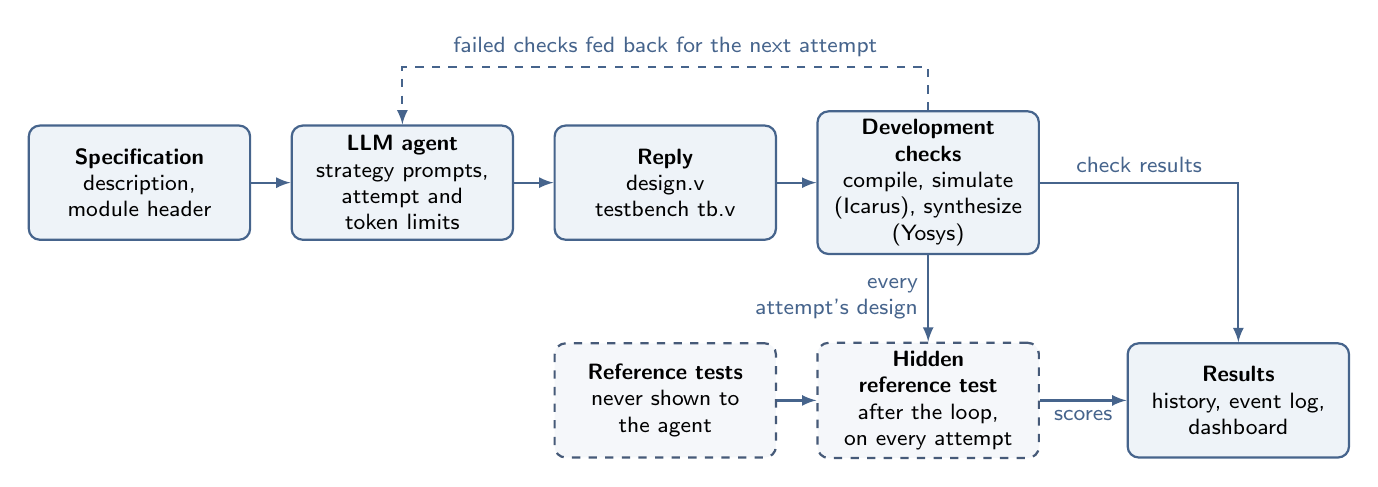
\begin{tikzpicture}[node distance=0.55cm and 0.5cm,
  box/.style={rectangle, rounded corners=4pt, draw=arrowcolor, fill=boxfill, thick, align=center,
    font=\sffamily\footnotesize, minimum height=1.45cm, text width=2.6cm, inner sep=3pt},
  hidden/.style={box, draw=secondary, fill=accent, dashed},
  flow/.style={->, >=latex, draw=arrowcolor, thick},
  back/.style={->, >=latex, draw=arrowcolor, thick, dashed}]
  \node[box] (spec) {\textbf{Specification}\\description,\\module header};
  \node[box, right=of spec] (llm) {\textbf{LLM agent}\\strategy prompts,\\attempt and\\token limits};
  \node[box, right=of llm] (files) {\textbf{Reply}\\design.v\\testbench tb.v};
  \node[box, right=of files] (dev) {\textbf{Development}\\\textbf{checks}\\compile, simulate\\(Icarus), synthesize\\(Yosys)};
  \node[hidden, below=1.1cm of dev] (ref) {\textbf{Hidden}\\\textbf{reference test}\\after the loop,\\on every attempt};
  \node[hidden, left=of ref] (refdata) {\textbf{Reference tests}\\never shown to\\the agent};
  \node[box, right=1.1cm of ref] (out) {\textbf{Results}\\history, event log,\\dashboard};
  \draw[flow] (spec) -- (llm);
  \draw[flow] (llm) -- (files);
  \draw[flow] (files) -- (dev);
  \draw[back] (dev.north) -- ++(0,0.55) -| node[pos=0.25, above, font=\footnotesize, color=arrowcolor]
    {failed checks fed back for the next attempt} (llm.north);
  \draw[flow] (dev) -- node[left, font=\footnotesize, color=arrowcolor, align=right] {every\\attempt's design} (ref);
  \draw[flow] (refdata) -- (ref);
  \draw[flow] (ref) -- node[below, font=\footnotesize, color=arrowcolor] {scores} (out);
  \draw[flow] (dev.east) -| node[pos=0.25, above, font=\footnotesize, color=arrowcolor] {check results} (out.north);
\end{tikzpicture}
\caption{The agent loop. Only the development checks reach the model; the hidden reference test scores the designs
after the loop ends.}
\label{fig:loop}
\end{figure}

\todo{The loop (Figure~\ref{fig:loop}): the \texttt{single} workflow (one reply holds design and testbench) and
\texttt{spec\_first} (the testbench is written from the specification first, in its own conversation, and its author
reviews disputed checks). Limits: \fact{max-attempts} attempts, \fact{budget} tokens. What the development checks
report back. Every run keeps its event log, history and the prompts it used.}

\subsection{Keeping the evaluation honest}
\todo{Hidden reference tests are written by the team and stay outside the agent's view; each run replaces their
result-line placeholder with a random token, so generated code cannot print a fake pass. Each attempt is scored
after the loop, so one run gives a paired one-shot (attempt 1) and iterative (final) score. The tools run with
timeouts and capped output. The \fact{fixtures} fixtures (\fact{fixtures-correct} correct, the rest deliberately
faulty) check the tests themselves (\texttt{docs/acceptance-checks.md}).}

\subsection{Circuits}
\begin{table}[H]
\centering\small
\begin{tabular}{l l l r r}
\toprule
Circuit & Family & Split & \makecell{Hidden-test\\checks} & \makecell{Fixtures\\correct / faulty} \\
\midrule
\texttt{adder4} & adder & Dev & 512 & 2 / 3 \\
\texttt{mux2} & mux & Dev & 524 & 2 / 4 \\
\texttt{counter4} & counter & Dev & 249 & 2 / 4 \\
\texttt{alu4} & alu & Dev & 2,048 & 2 / 5 \\
\texttt{seqdet\_moore} & fsm & Dev & 686 & 2 / 4 \\
\texttt{adder8} & adder & Held-out & 131,072 & 2 / 3 \\
\texttt{mux4} & mux & Held-out & 1,064 & 2 / 3 \\
\texttt{updown8} & counter & Held-out & 380 & 2 / 4 \\
\texttt{alu8} & alu & Held-out & 524,288 & 2 / 4 \\
\texttt{seqdet\_mealy} & fsm & Held-out & 684 & 2 / 4 \\
\bottomrule
\end{tabular}

\caption{The \fact{circuits} circuits. Strategies were tuned on the dev circuits only; the held-out circuits were used
once per strategy, with the runs declared in advance.}
\label{tab:circuits}
\end{table}

% ============================================================================
\section{The toolkit}

\todo{What a student does with it, by dashboard section: (1) pick a circuit, strategy, mode and model; (2) watch the
run live; (3) inspect every attempt: design, testbench, changes from the previous attempt, the hidden test's
mismatches, waveforms, the feedback the model got, and editing the RTL to re-test it; (4) benchmark charts;
(5) the strategy editor. Exports. Then delivery: Docker image with pinned tool versions, Compose with Ollama on the
GPU, the image published by CI after its tests pass.}

\shot{Running the agent: inputs and the live log.}{sections 1 and 2 during a gemma4 run}
\shot{One attempt in the results view, with the waveform of a failing hidden test.}{section 3, Waveform tab, alu8 SLT bug}
\shot{Editing an attempt's RTL and re-testing it.}{section 3, Edit \& re-test tab with the signed-comparison fix}
\shot{Benchmark charts.}{section 4, held-out benchmark}

% ============================================================================
\section{Experimental method}

\todo{Model \fact{model} through Ollama, temperature \fact{temperature}, fixed seeds \fact{seeds} (the same seed
reproduced a run exactly at this temperature). Up to \fact{max-attempts} attempts and \fact{budget} tokens per run.
Four strategies: \texttt{default} (the baseline, unchanged), \texttt{tb\_timing}, \texttt{spec\_first} v1 and v2.
Every attempt scored, so one-shot and iterative come from the same runs (paired). Metrics as promised in the
proposal: compilation, hidden-test pass rate, synthesis, retries, latency and tokens; cell counts only for passing
designs under the same Yosys flow. Order of work: tune on dev, declare, run held-out once, no tuning after.}

% ============================================================================
\section{Results}

\begin{table}[H]
\centering\small\setlength{\tabcolsep}{4.5pt}
\begin{tabular}{l rrrr c r rr}
\toprule
Strategy & One-shot & Iterative & Fixed & Broken & \makecell{Pass after\\1 / 2 / 3} & \makecell{Own checks\\reject correct} & \makecell{Mean\\tokens} & \makecell{Mean\\time} \\
\midrule
\multicolumn{9}{l}{\textit{Held-out circuits}} \\
default & 22/25 & \up{24/25} & 2 & 0 & 22 / 24 / 24 & 81\% & 10,501 & 23.7\,s \\
tb\_timing & 25/25 & 25/25 & 0 & 0 & 25 / 25 / 25 & 54\% & 6,780 & 18.3\,s \\
spec\_first v1 & 20/25 & \up{21/25} & 2 & 1 & 20 / 21 / 21 & 65\% & 12,526 & 26.1\,s \\
spec\_first v2 & 20/25 & \up{23/25} & 3 & 0 & 20 / 23 / 23 & 59\% & 12,817 & 25.9\,s \\
\midrule
\multicolumn{9}{l}{\textit{Dev circuits}} \\
default & 24/25 & 24/25 & 0 & 0 & 24 / 24 / 24 & 51\% & 7,296 & 16.6\,s \\
tb\_timing & 23/25 & \down{22/25} & 0 & 1 & 23 / 22 / 22 & 36\% & 5,906 & 15.9\,s \\
spec\_first v1 & 23/25 & \up{24/25} & 1 & 0 & 23 / 24 / 24 & 21\% & 5,985 & 15.4\,s \\
spec\_first v2 & 23/25 & 23/25 & 2 & 2 & 23 / 24 / 23 & 32\% & 6,744 & 15.6\,s \\
\bottomrule
\end{tabular}

\caption{One-shot vs.\ iterative, per strategy and split (25 runs each). \up{Green}: revising helped overall;
\down{red}: it hurt. ``Own checks reject correct'': share of correct designs (by the hidden test) that the agent's
own development checks failed.}
\label{tab:strategy}
\end{table}

\begin{figure}[H]
\centering
\begin{tikzpicture}
\foreach \split/\name [count=\i] in {heldout/Held-out, dev/Dev} {
  \begin{axis}[at={(\i*7.6cm-7.6cm,0)}, width=7.2cm, height=5.2cm, title={\name\ circuits},
      xlabel={stopped after attempt}, ylabel={runs passing (of 25)}, xtick={1,2,3}, ymin=17.5, ymax=25.5,
      ytick={18,20,22,24,25}, legend style={font=\scriptsize, at={(0.03,0.03)}, anchor=south west},
      every axis plot/.append style={thick, mark size=2pt}, tick label style={font=\footnotesize},
      label style={font=\footnotesize}, title style={font=\small\bfseries}]
    \addplot[color=primary, mark=*] table[x=attempt, y=default, col sep=comma] {generated/pass-after-\split.csv};
    \addplot[color=good, mark=square*] table[x=attempt, y=tbtiming, col sep=comma] {generated/pass-after-\split.csv};
    \addplot[color=orange, mark=triangle*] table[x=attempt, y=sfone, col sep=comma] {generated/pass-after-\split.csv};
    \addplot[color=bad, mark=diamond*] table[x=attempt, y=sftwo, col sep=comma] {generated/pass-after-\split.csv};
    \ifnum\i=2 \legend{default, tb\_timing, spec\_first v1, spec\_first v2}\fi  % dev panel: its lower left is empty
  \end{axis}}
\end{tikzpicture}
\caption{Hidden-test passes if each run had stopped after 1, 2 or 3 attempts (attempt 1 is the one-shot result).
The vertical axis starts at 17.5.}
\label{fig:pass-after}
\end{figure}

\begin{table}[H]
\centering\small
\begin{tabular}{l c c c c r}
\toprule
Circuit & default & tb\_timing & spec\_first v1 & spec\_first v2 & Median cells \\
\midrule
\texttt{adder8} & 5 & 5 & 5 & 5 & 52 \\
\texttt{mux4} & \up{3 $\to$ 5} & 5 & 5 & 5 & 15 \\
\texttt{updown8} & 5 & 5 & \down{5 $\to$ 4} & 5 & 47 \\
\texttt{alu8} & 4 & 5 & 4 & 4 & 256 \\
\texttt{seqdet\_mealy} & 5 & 5 & \up{1 $\to$ 3} & \up{1 $\to$ 4} & 9 \\
\bottomrule
\end{tabular}

\caption{Held-out circuits: passing runs out of 5, one-shot $\to$ iterative, and the median cell count of passing final
designs.}
\label{tab:circuits-heldout}
\end{table}

\begin{table}[H]
\centering\small
\begin{tabular}{l c c c c r}
\toprule
Circuit & default & tb\_timing & spec\_first v1 & spec\_first v2 & Median cells \\
\midrule
\texttt{adder4} & 5 & 5 & 5 & 5 & 23 \\
\texttt{mux2} & 5 & 5 & 5 & 5 & 8 \\
\texttt{counter4} & 5 & 5 & 5 & \down{5 $\to$ 3} & 10 \\
\texttt{alu4} & 4 & \down{4 $\to$ 3} & \up{3 $\to$ 4} & \up{3 $\to$ 5} & 134 \\
\texttt{seqdet\_moore} & 5 & 4 & 5 & 5 & 18 \\
\bottomrule
\end{tabular}

\caption{Dev circuits, as in Table~\ref{tab:circuits-heldout}.}
\label{tab:circuits-dev}
\end{table}

\subsection{How reliable were the agent's own checks?}

\begin{figure}[H]
\centering
\begin{tikzpicture}
\begin{axis}[ybar, bar width=9pt, width=12cm, height=5cm, ymin=0, ymax=100, ylabel={correct designs rejected (\%)},
    symbolic x coords={default,tbtiming,sfone,sftwo}, xtick=data,
    xticklabels from table={generated/own-checks.csv}{label}, table/col sep=comma,
    nodes near coords, nodes near coords style={font=\scriptsize}, legend columns=2,
    legend style={font=\scriptsize, at={(0.5,1.03)}, anchor=south, draw=none},
    tick label style={font=\footnotesize}, label style={font=\footnotesize}, enlarge x limits=0.18]
  \addplot[fill=primary!80, draw=primary] table[x=strategy, y=heldout, col sep=comma] {generated/own-checks.csv};
  \addplot[fill=secondary!35, draw=secondary] table[x=strategy, y=dev, col sep=comma] {generated/own-checks.csv};
  \legend{held-out, dev}
\end{axis}
\end{tikzpicture}
\caption{Share of correct designs (passing the hidden test) that the agent's own development checks rejected, over
all attempts.}
\label{fig:own-checks}
\end{figure}

\begin{table}[H]
\centering\small
\begin{tabular}{l rr rr}
\toprule
& \multicolumn{2}{c}{Correct designs rejected} & \multicolumn{2}{c}{Wrong designs accepted} \\
\cmidrule(lr){2-3}\cmidrule(lr){4-5}
Strategy & count & share & count & share \\
\midrule
\multicolumn{5}{l}{\textit{Held-out circuits}} \\
default & 47 of 58 & 81\% & 0 of 5 & 0\% \\
tb\_timing & 22 of 41 & 54\% & none & -- \\
spec\_first v1 & 24 of 37 & 65\% & 2 of 11 & 18\% \\
spec\_first v2 & 22 of 37 & 59\% & 1 of 8 & 12\% \\
\midrule
\multicolumn{5}{l}{\textit{Dev circuits}} \\
default & 20 of 39 & 51\% & 0 of 3 & 0\% \\
tb\_timing & 12 of 33 & 36\% & 2 of 6 & 33\% \\
spec\_first v1 & 6 of 29 & 21\% & 1 of 2 & 50\% \\
spec\_first v2 & 10 of 31 & 32\% & 1 of 5 & 20\% \\
\bottomrule
\end{tabular}

\caption{The agent's own checks against the hidden test, over all scored attempts.}
\label{tab:own-checks}
\end{table}

\begin{table}[H]
\centering\small\setlength{\tabcolsep}{5pt}
\begin{tabular}{l r rr rr}
\toprule
& & \multicolumn{2}{c}{Right call} & \multicolumn{2}{c}{Wrong call} \\
\cmidrule(lr){3-4}\cmidrule(lr){5-6}
Version & Reviews & \makecell{revised,\\design correct} & \makecell{kept,\\design wrong} & \makecell{kept,\\design correct} & \makecell{revised,\\design wrong} \\
\midrule
\multicolumn{6}{l}{\textit{Held-out circuits}} \\
spec\_first v1 & 28 & 15 & 1 & 9 & 3 \\
spec\_first v2 & 26 & 6 & 1 & 18 & 1 \\
\midrule
\multicolumn{6}{l}{\textit{Dev circuits}} \\
spec\_first v1 & 12 & 10 & 0 & 0 & 2 \\
spec\_first v2 & 14 & 1 & 3 & 10 & 0 \\
\bottomrule
\end{tabular}

\caption{\texttt{spec\_first}: testbench reviews after a design failed some checks, judged by the hidden test of the
design under review.}
\label{tab:reviews}
\end{table}

\todo{Walk the reader through the tables: revising fixed \fact{fixed} and broke \fact{broken} of \fact{runs} paired runs;
on held-out, \texttt{default} went \fact{heldout-default-oneshot} $\to$ \fact{heldout-default-final} and
\texttt{spec\_first} v2 \fact{heldout-sftwo-oneshot} $\to$ \fact{heldout-sftwo-final}; over both splits the strategies
score \fact{both-final-range} and their order flips between splits. Own
checks rejected \fact{heldout-rejected-range} of correct held-out designs (\fact{dev-rejected-range} on dev). Cost:
iterative runs used several times the one-shot tokens.}

% ============================================================================
\section{Discussion}

\todo{What iteration fixes: errors the tools name (compile errors, e.g.\ assigning a non-reg output in an always
block). What it does not fix: specification-level logic bugs (the unsigned SLT comparison survived every revision).
Why: the model's testbench shares the design's misconception, has timing bugs, or rejects correct designs, so the
feedback is often wrong (the proposal's ``biggest roadblock''). The \texttt{spec\_first} result: separating the
testbench author reduced false rejections on dev but not on held-out. Strategy differences are within run-to-run
noise at 25 runs per cell. Examples from the benchmark report (docs/benchmark-report.html).}

% ============================================================================
\section{Limitations and threats to validity}

\todo{Five seeds per setting; one model; small circuits; reference tests written by the team (checked by fixtures,
but not proofs); cell counts are not power, area or timing; GPU nondeterminism; RAG and LoRA fine-tuning (stretch
goals) not attempted.}

% ============================================================================
\section{Reproducibility}

\todo{The repository (github.com/Harrydhara/VLSI-Design-Agentic-Framework), the image
(ghcr.io/harrydhara/vlsi-design-agentic-framework) with pinned versions (Icarus Verilog 12, Yosys 0.57+260 built from
the benchmark commit, Ollama 0.31.2, exact Python packages). Commands: rerun a benchmark (\texttt{vlsi-agent bench}),
regenerate these tables (\texttt{generate.py}), and the HTML report. All runs behind this report are committed under
\texttt{runs/bench/}.}

% ============================================================================
\section{Deliverables against the proposal}

\todo{One table: each proposal promise (MVP, dashboard features, evaluation, final deliverables) and each member's
completion check from the division of work, with the evidence (docs/acceptance-checks.md: all three checks pass) and
any gaps (RAG and LoRA not attempted; an FPGA board was optional and not used).}

% ============================================================================
\section{Conclusion and future work}

\todo{The answer to the research question in two sentences. Future work: better testbench feedback (a harness that
samples at the right moment), RAG over Verilog examples, LoRA fine-tuning with separate data, multi-agent review, larger
circuits (a FIFO pair), delivering the last compiling design.}

% ============================================================================
\appendix
\section{A worked example: the unsigned SLT bug}

\todo{One run end to end (runs/bench/heldout-seeds1-5/runs/alu8/default/seed4): the specification, the design's
9-bit sign-extended but unsigned comparison, the own testbench's verdict, the feedback, three unchanged attempts, the
hidden test's mismatches and waveform, and the one-word manual fix that passes 524,288/524,288
(runs/manual/20261020-141335-alu8-edit) while the model's testbench still reports 0/22.}

\section{The baseline prompts}

The \texttt{default} strategy, unchanged throughout the project.

\textbf{system.txt}
\VerbatimInput[fontsize=\scriptsize, frame=single, rulecolor=\color{border}, breaklines]{generated/prompt-system.txt}

\textbf{task.txt}
\VerbatimInput[fontsize=\scriptsize, frame=single, rulecolor=\color{border}, breaklines]{generated/prompt-task.txt}

\textbf{feedback.txt}
\VerbatimInput[fontsize=\scriptsize, frame=single, rulecolor=\color{border}, breaklines]{generated/prompt-feedback.txt}

\end{document}
